\documentclass[documentation.tex]{subfiles}
\begin{document}
	Il videogioco è stato sviluppato utilizzando la IDE Unity3D. Gli script inseriti nel progetto e riportati nel documento sono scritti nel linguaggio CSharp. Come ogni progetto sviluppato in Unity3D, questo è suddiviso in scenes che sono dei blocchi funzionali, ciascuno con le proprie funzionalità e contenente i propri oggetti e script.
	\subsubsection{Struttura}
	Il progetto è suddiviso in 4 scenes.
		\paragraph{Welcome scene}
			\begin{itemize}
				\item Consente di scegliere tra la Game scene e la View Circuit scene
				\item Avvia la registrazione del circuito
				\item Consente di scegliere una lunghezza media del percorso che verrà costruito
			\end{itemize}
			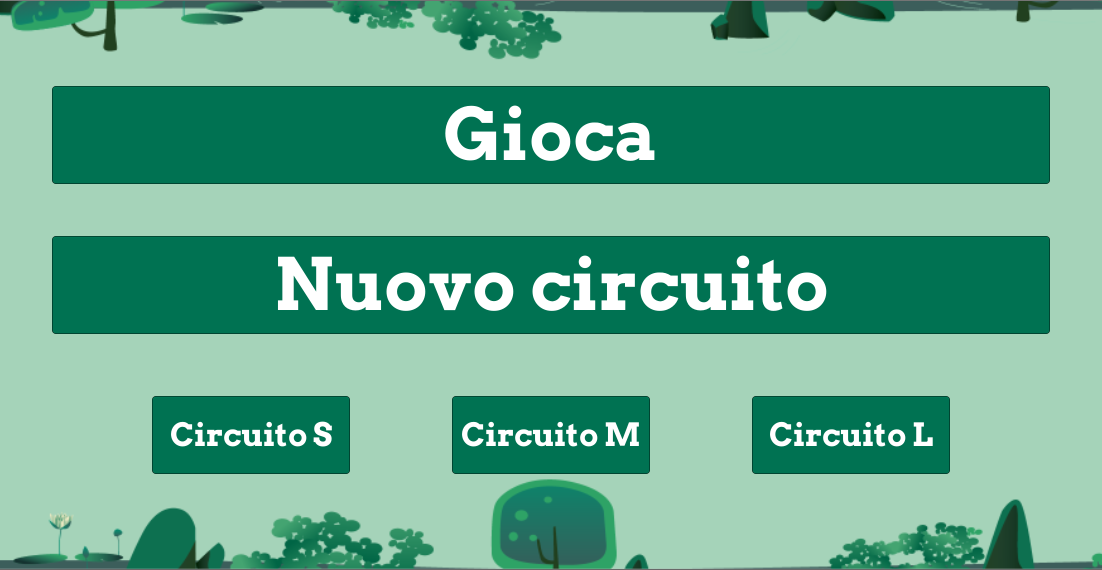
\includegraphics[width=\textwidth]{./images/welcome.png}
		\paragraph{Circuit Registration scene}
			\begin{itemize}
				\item Avvia la comunicazione tra tablet e giocattolo e la ricezione delle misure inviate da quest'ultimo
				\item Rielabora e filtra i dati ricevuti
				\item Avvia una delle due scenes finali
			\end{itemize}
			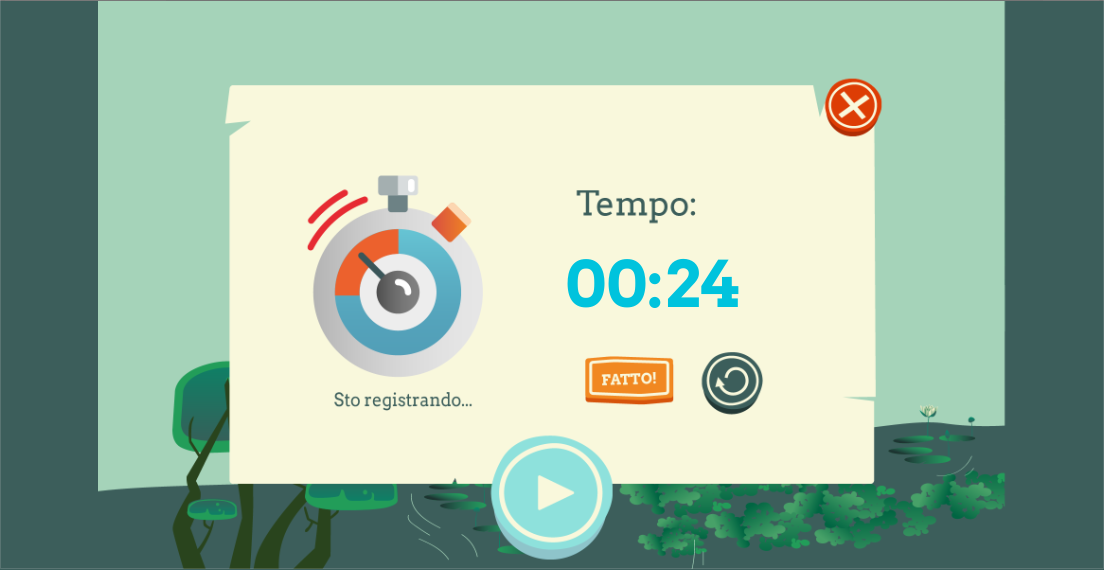
\includegraphics[width=\textwidth]{./images/countdown.png}
		\paragraph{Game scene}
			\begin{itemize}
				\item Costruisce il circuito digitale
				\item Avvia e gestisce la fase di gioco
			\end{itemize}
			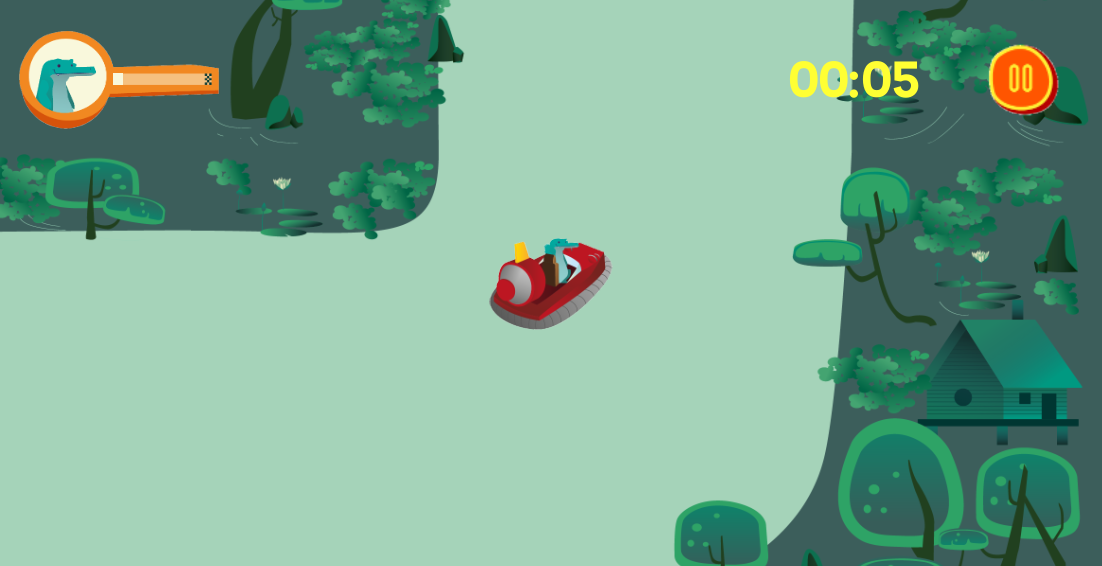
\includegraphics[width=\textwidth]{./images/game.png}
		\paragraph{View Circuit scene}
			\begin{itemize}
				\item Costruisce il circuito digitale
				\item Consente di visualizzare il circuito appena costruito nella sua interezza
			\end{itemize}
			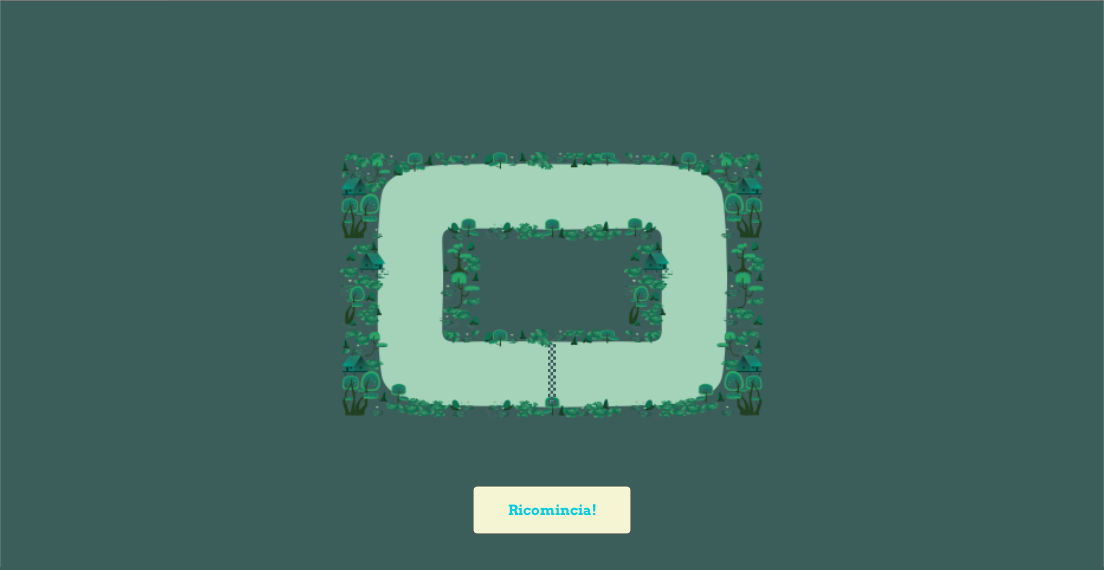
\includegraphics[width=\textwidth]{./images/view.png}
	\subsubsection{Ricezione delle misure}
		Questa funzionalità viene gestita nella seconda scene (Circuit Registration) e sono tre le principali classi che vengono interpellate:
		\begin{itemize}
			\item \textbf{WilDataManager:} Interagisce con la GUI e avvia sia la connessione con il giocattolo(e la successiva ricezione delle misure da parte della scheda che contiene) che il timeout.
			\item \textbf{CountdownManager:} Controlla il timer e notifica la classe principale(WilDataManager) quando la finestra temporale di ricezione delle misure da parte del giocattolo si è esaurita.
			\item \textbf{MeasureManager: } Esegue la connessione TCP con la scheda e legge e salva le misurazioni che vengono inviate da quest'ultima; quando il tempo di ricezione delle misure è scaduto termina la connessione e invia le misure ricevute alla classe principale(WilDataManager)
		\end{itemize}
		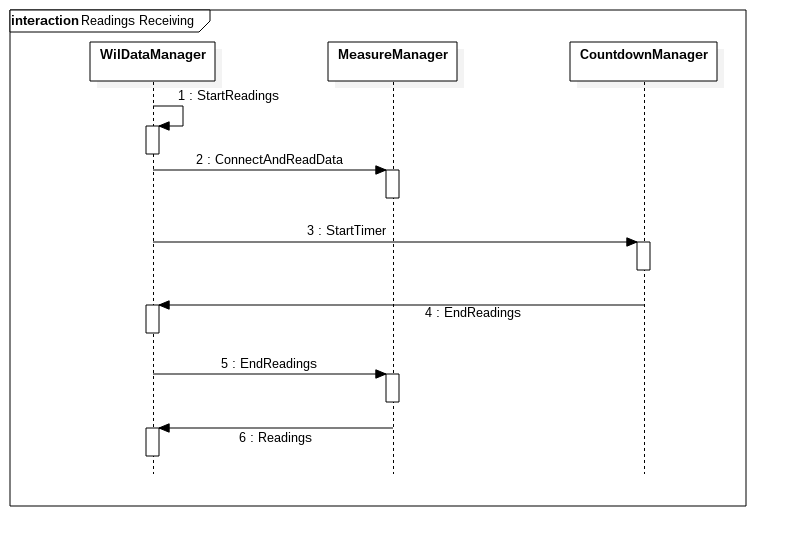
\includegraphics[width=\textwidth]{./diagrams/measure_receiving.png}
	\subsubsection{filtraggio e rielaborazione dei dati}
		Una volta ricevute le misure da parte del giocattolo è necessario rielaborarle affinchè si possa ricostruire il percorso compiuto fisicamente a livello digitale. Ricevute le varie accelerazioni effettuate delle scheda è dunque necessario decifrare come la scheda si è spostata nello spazio. Tutte le trasformazioni necessarie vengono eseguite nella classe \textit{WilDataManager} nel metodo \textit{ElaborateEntries()}, una volta terminata la comunicazione con il giocattolo. I dati vengono inizialmente filtrati, dopodichè viene eseguita una trasformazione delle misure di accelerazione in motion detection.
		\paragraph{Filtraggio}Per raffinare i dati ricevuti e renderli meno soggetti ad errore, questi vengono filtrati attraverso un filtro passa-basso. Il filtro legge tutte le misure ricevute e, basandosi sulla misura in esame e quella precedente, modifica la misura secondo la relazione:
		\begin{center}
		$m_{i} = factor * m_{i} + (1 - factor) * m_{i-1}, factor \in [0,1]$
		\end{center}
		\textit{factor} è un valore ottenuto sperimentalmente confrontando l'effetto di alcuni suoi valori sulla precisione della misura effettuata. Un valore vicino allo 0 tende ad "appiattire" tutte le misure di accelerazione ottenute sull'asse 0, mentre un valore di factor pari a 1 non induce alcuna modifica sulle misure ricevute.
		\paragraph{Motion Detection} Viene definita una certa \textit{soglia} che separa i dati interessanti da quelli trascurabili. Se una misura di accelerazione è inferiore a tale soglia(in valore assoluto), allora tale misura è trascurabile, nel senso che è dovuta a un errore di misurazione o che è dovuta a uno spostamento trascurabile del giocattolo. Il valore della soglia influenza la sensibilità allo spostamento della scheda. Confrontare le misure di accelerazione lungo un certo asse(x,y) con la soglia consente di stabilire se tale misura corrisponde a uno spostamento del giocattolo lungo tale asse(+1 o -1) o se il giocattolo è rimasto fermo(0). Il movimento del giocattolo viene quindi approssimato come una sequenza di spostamenti, ciascuno lungo 8 possibili direzioni(N, NE, E, SE, S, SW, W, NW).\\
		Sia threshold il valore della soglia, siano xList e yList liste di valori che rappresentano le misure di accelerazione lungo gli assi x e y(il cui valore è confrontabile con quello di threshold) e siano moveX e moveY le relative liste di dati di motion detection:
		\lstset{style=csharp}
		\begin{lstlisting}
int movex, movey;

// convert data into motion detection values
for (i = 0; i < xList.Count; i++) {
	// movex
	if (xList [i] > threshold) {
		movex = 1;
	} else if (xList [i] < -threshold) {
		movex = -1;
	} else {
		movex = 0;
	}
	//movey
	if (yList [i] > threshold) {
		movey = 1;
	} else if (yList [i] < -threshold) {
		movey = -1;
	} else {
		movey = 0;
	}
	moveX.Add (movex);
	moveY.Add (movey);
}
		\end{lstlisting}
		\paragraph{Ulteriori rielborazioni} Affinchè sia possibile costruire il percorso a partire dai nuovi dati ottenuti nelle liste moveX e moveY, questi devono essere rielaborati. In particolare:
		\begin{itemize}
			\item Vengono eliminati tutti i punti che non provocano alcuna modifica nella costruzione del percorso(gli spostamenti 0,0). Questi punti sono i valori j per cui moveX[j] e moveY[j] sono entrambi nulli.
			\item Vengono eliminati tutti gli spostamenti che sono opposti a quelli precedenti. Questi spostamenti indurrebbero il percorso a "ritornare sui propri passi", che è un comportamento difficile da gestire. Spesso questo comportamento è conseguenza di un errore di misura. Per ogni spostamento (moveX[j], moveY[j]) vengono eliminati i successivi spostamenti ruotati di 180 gradi rispetto al j-esimo,cioè  tutti i k per cui moveX[j] + moveX[k] = 0 e moveY[j] + moveY[k] = 0.
		\end{itemize}
		\paragraph{Posizione} Una volta raffinati tutti gli spostamenti nelle liste moveX e moveY, vengono calcolate le liste posX e posY che rappresentano la posizione nello spazio del giocattolo in seguito ad ogni spostamento. Il percorso inizia sempre in posizione (0,0). Nel caso in cui uno spostamento imponesse una posizione in un punto già raggiunto in precedenza(il percorso avrebbe degli overlapping), tale spostamento viene ignorato.
		\begin{lstlisting}
posX.Add (0);
posY.Add (0);
int lastx = 0;
int lasty = 0;
int px = 0;
int py = 0;

for (i = 0; i < moveX.Count; i++) {
	px = lastx + moveX [i];
	py = lasty + moveY [i];
	if (!PointAlreadyPresent(posX, posY, px, py)) {
		// no overlapping point
		posX.Add (px);
		posY.Add (py);
		lastx = px;
		lasty = py;
	}
}
		\end{lstlisting}
		Il grafico ottenuto da (posX, posY) è l'approssimazione del movimento del giocattolo con cui verrà costruito il percorso digitale.
		
	\subsubsection{Creazione del percorso}
	La prima fase della scene \textit{Game} è quello di costruire il circuito in cui far giocare l'utente. Questa funzionalità è gestita dalla classe \textit{DataManager}. Partendo dalla lista di posizione calcolata nella fase di registrazione del percorso, viene generato il circuito vero e proprio generando una lista di tiles predefinite che posizionate una dopo l'altra ricalchino il percorso registrato. Le tiles gestiscono gli spostamenti nelle 8 direzioni e in più sono previste delle curve a 90 gradi affinchè ciascuna possa essere collegata alle altre. L'algoritmo ad alto livello che viene seguito è il seguente:
	\begin{enumerate}
		\item Viene disegnata la tile iniziale che comprende la start flag;
		\item Per ogni punto presente nella lista di posizione viene valutato se è necessario disegnare una tile di curva per collegare la tile precedente a quella successiva, dopodichè viene disegnata la tile successiva;
		\item Viene disegnata la tile finale che comprende la finish flag.
	\end{enumerate}
	Di seguito è riportato un esempio di circuito costruito a partire da una lista di punti:
	\begin{figure}[h]
	\subfloat{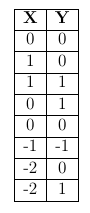
\includegraphics[scale=0.8]{./images/table.png}}
	\subfloat{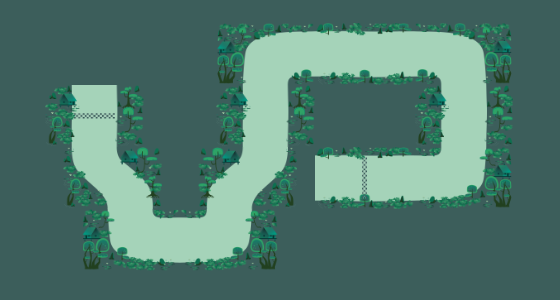
\includegraphics[scale=0.8]{./images/path.png}}
	\end{figure}
\end{document}